% This file was converted to LaTeX by Writer2LaTeX ver. 1.0.2
% see http://writer2latex.sourceforge.net for more info
\documentclass[a4paper]{article}
\usepackage[ascii]{inputenc}
\usepackage[T1]{fontenc}
\usepackage[english,spanish]{babel}
\usepackage{amsmath}
\usepackage{amssymb,amsfonts,textcomp}
\usepackage{color}
\usepackage{array}
\usepackage{hhline}
\usepackage{hyperref}
\hypersetup{pdftex, colorlinks=true, linkcolor=blue, citecolor=blue, filecolor=blue, urlcolor=blue, pdftitle=, pdfauthor=, pdfsubject=, pdfkeywords=}
\usepackage[pdftex]{graphicx}
% Text styles
\newcommand\textstyleStrongEmphasis[1]{\textbf{#1}}
\newcommand\textstyleEmphasis[1]{\textit{#1}}
% Outline numbering
\setcounter{secnumdepth}{0}
% List styles
\newcommand\liststyleLxi{%
\renewcommand\labelitemi{{\textbullet}}
\renewcommand\labelitemii{{\textbullet}}
\renewcommand\labelitemiii{{\textbullet}}
\renewcommand\labelitemiv{{\textbullet}}
}
\newcommand\liststyleLx{%
\renewcommand\theenumi{\arabic{enumi}}
\renewcommand\theenumii{\arabic{enumii}}
\renewcommand\theenumiii{\arabic{enumiii}}
\renewcommand\theenumiv{\arabic{enumiv}}
\renewcommand\labelenumi{\theenumi.}
\renewcommand\labelenumii{\theenumii.}
\renewcommand\labelenumiii{\theenumiii.}
\renewcommand\labelenumiv{\theenumiv.}
}
\newcommand\liststyleLix{%
\renewcommand\labelitemi{{\textbullet}}
\renewcommand\labelitemii{{\textbullet}}
\renewcommand\labelitemiii{{\textbullet}}
\renewcommand\labelitemiv{{\textbullet}}
}
\newcommand\liststyleLviii{%
\renewcommand\theenumi{\arabic{enumi}}
\renewcommand\theenumii{\arabic{enumii}}
\renewcommand\theenumiii{\arabic{enumiii}}
\renewcommand\theenumiv{\arabic{enumiv}}
\renewcommand\labelenumi{\theenumi.}
\renewcommand\labelenumii{\theenumii.}
\renewcommand\labelenumiii{\theenumiii.}
\renewcommand\labelenumiv{\theenumiv.}
}
\newcommand\liststyleLvii{%
\renewcommand\theenumi{\arabic{enumi}}
\renewcommand\theenumii{\arabic{enumii}}
\renewcommand\theenumiii{\arabic{enumiii}}
\renewcommand\theenumiv{\arabic{enumiv}}
\renewcommand\labelenumi{\theenumi.}
\renewcommand\labelenumii{\theenumii.}
\renewcommand\labelenumiii{\theenumiii.}
\renewcommand\labelenumiv{\theenumiv.}
}
\newcommand\liststyleLi{%
\renewcommand\labelitemi{{\textbullet}}
\renewcommand\labelitemii{{\textbullet}}
\renewcommand\labelitemiii{{\textbullet}}
\renewcommand\labelitemiv{{\textbullet}}
}
\newcommand\liststyleLxii{%
\renewcommand\labelitemi{{\textbullet}}
\renewcommand\labelitemii{{\textbullet}}
\renewcommand\labelitemiii{{\textbullet}}
\renewcommand\labelitemiv{{\textbullet}}
}
\newcommand\liststyleLxiii{%
\renewcommand\labelitemi{{\textbullet}}
\renewcommand\labelitemii{{\textbullet}}
\renewcommand\labelitemiii{{\textbullet}}
\renewcommand\labelitemiv{{\textbullet}}
}
\newcommand\liststyleLxiv{%
\renewcommand\theenumi{\arabic{enumi}}
\renewcommand\theenumii{\arabic{enumii}}
\renewcommand\theenumiii{\arabic{enumiii}}
\renewcommand\theenumiv{\arabic{enumiv}}
\renewcommand\labelenumi{\theenumi.}
\renewcommand\labelenumii{\theenumii.}
\renewcommand\labelenumiii{\theenumiii.}
\renewcommand\labelenumiv{\theenumiv.}
}
\newcommand\liststyleLxv{%
\renewcommand\labelitemi{{\textbullet}}
\renewcommand\labelitemii{{\textbullet}}
\renewcommand\labelitemiii{{\textbullet}}
\renewcommand\labelitemiv{{\textbullet}}
}
\newcommand\liststyleLxvi{%
\renewcommand\labelitemi{{\textbullet}}
\renewcommand\labelitemii{{\textbullet}}
\renewcommand\labelitemiii{{\textbullet}}
\renewcommand\labelitemiv{{\textbullet}}
}
% Page layout (geometry)
\setlength\voffset{-1in}
\setlength\hoffset{-1in}
\setlength\topmargin{2cm}
\setlength\oddsidemargin{2cm}
\setlength\textheight{25.7cm}
\setlength\textwidth{17.001cm}
\setlength\footskip{0.0cm}
\setlength\headheight{0cm}
\setlength\headsep{0cm}
% Footnote rule
\setlength{\skip\footins}{0.119cm}
\renewcommand\footnoterule{\vspace*{-0.018cm}\setlength\leftskip{0pt}\setlength\rightskip{0pt plus 1fil}\noindent\textcolor{black}{\rule{0.25\columnwidth}{0.018cm}}\vspace*{0.101cm}}
% Pages styles
\makeatletter
\newcommand\ps@Standard{
  \renewcommand\@oddhead{}
  \renewcommand\@evenhead{}
  \renewcommand\@oddfoot{}
  \renewcommand\@evenfoot{}
  \renewcommand\thepage{\arabic{page}}
}
\makeatother
\pagestyle{Standard}
\title{}
\author{}
\date{2015-09-27T17:26:35.118163052}
\begin{document}
\section[The making of MADE (Part 1): It{\textquoteright}s all about
backstories]{\href{http://www.velonuboso.com/made/2015/06/13/making-part-1-events-facts-deductions-backstories/}{The
making of MADE (Part 1): It{\textquoteright}s all about backstories}}
The aim of MADE is to create \textstyleStrongEmphasis{coherent and
interesting massive basktories in an open world context} that lead to a
\textstyleStrongEmphasis{more immersive and realistic game experience}.

Following the definition by the Wikipedia [1], the
\textstyleStrongEmphasis{backstory}, also called
\textstyleEmphasis{background story}, \textstyleEmphasis{back-story} or
\textstyleEmphasis{background}, is a
{\textquoteleft}\textstyleEmphasis{set of events invented for a plot,
presented as preceding and leading up to that plot. It is a literary
device of a narrative history all chronologically earlier than the
narrative of primary interest}{\textquoteright}.

Following this definition, creating the backstories of the inhabitants
of a virtual world consists on creating those events, that may contain
information about characters, places, actions, and time.

{\bfseries
References}

[1] Wikipedia contributors. (2015, June 13). Backstory [Online].
Available:
https://en.wikipedia.org/w/index.php?title=Backstory\&oldid=666312396


\bigskip

\clearpage\section[The making of MADE (Part 2): Events that tell
stories]{\href{http://www.velonuboso.com/made/2015/06/13/making-part-2-events-tells-stories/}{The
making of MADE (Part 2): Events that tell stories}}
June 13, 2015

Kim [1] theorized that the term
{\textquoteleft}\textstyleEmphasis{event}{\textquoteright}
usually~implies a change, and most changes are changes in a
\textstyleEmphasis{substance} (an individual, an object, a living thing
or a system), that occur when {\textquoteleft}\textstyleEmphasis{it
acquires a property it did not previously have, or loses a property it
previously had}{\textquoteright}. Formerly, Kim defined the events in
his \textstyleStrongEmphasis{theory of the structured complexes} using
the canonical notation \textstyleEmphasis{[x, P, t]}, where
\textstyleEmphasis{x} is the \textstyleEmphasis{substance},
\textstyleEmphasis{P} is the \textstyleEmphasis{property} it
exemplifies and \textstyleEmphasis{t} is the time. The
\textstyleStrongEmphasis{existence condition} implies that
\textstyleEmphasis{Event [x, P, t]} exists just in case that substance
\textstyleEmphasis{x} has the property \textstyleEmphasis{P} at the
time \textstyleEmphasis{t}.

\textstyleStrongEmphasis{In MADE, the events that compound the
backstories are defined as meaningful logical predicates} with
notation~Predicate(t,x[200B?]0[200B?][200B?],/dots,x[200B?]n[200B?][200B?])~where
\textstyleEmphasis{t} is the time, and each \textstyleEmphasis{x} is an
element of the world (a character, a cell, a time, the property of an
element or a value). Each predicate has a
\textstyleStrongEmphasis{name}, a \textstyleStrongEmphasis{signature}
(or arguments) and an \textstyleStrongEmphasis{interpretation}, that is
a description of the event in natural language.

\textstyleEmphasis{For instance, the classical predicate Born could be
defined
as~Born(t,x[200B?]0[200B?][200B?],x[200B?]1[200B?][200B?],x[200B?]2[200B?][200B?])~where
t is the time, x[200B?]0[200B?][200B?] is the character that has born,
~x[200B?]1[200B?][200B?] is his/her father and~x[200B?]2[200B?][200B?]
is his/her mother.~The predicate has a name, a signature and an
interpretation
({\textquotedblleft}{\textless}x[200B?]0[200B?][200B?]{\textgreater}
was born in {\textless}t{\textgreater}. His/her father was
{\textless}x[200B?]1[200B?][200B?]{\textgreater} and his/her mother was
{\textless}x[200B?]2[200B?][200B?]{\textgreater}{\textquotedblright}).}

{\bfseries
References:}

[1] Kim, Jaegwon, {\textquotedblleft}Events as Property
Exemplifications{\textquotedblright} in Action Theory, ser. Synthese
Library, M. Brand and D. Walton, Eds., 1976, vol. 97.


\bigskip

\clearpage\section[The making of MADE (Part 3): world{\textquoteright}s
facts, world{\textquoteright}s deductions and world{\textquoteright}s
backstories]{\href{http://www.velonuboso.com/made/2015/06/14/making-part-3-worlds-facts-worlds-deductions-worlds-backstories/}{The
making of MADE (Part 3): world{\textquoteright}s facts,
world{\textquoteright}s deductions and world{\textquoteright}s
backstories}}
June 14, 2015

In MADE, the collection of events generated in the virtual world and
that relate to all the characters is called the
\textstyleStrongEmphasis{world{\textquoteright}s facts}. As they are
expressed as logical predicates, \textstyleStrongEmphasis{deductive
reasoning mechanisms can be used to extract knowledge from the world}.
As opposed to the \textstyleStrongEmphasis{world{\textquoteright}s
facts}, the collection of deduction rules and Predicates is called the
\textstyleStrongEmphasis{world{\textquoteright}s deductions}.

Deductions can be expressed as
Expression[200B?]0[200B?][200B?]$\rightarrow
$Expression[200B?]1[200B?][200B?], where
Expression[200B?]0[200B?][200B?]~is the premise and
Expression[200B?]1[200B?][200B?]~the conclusion, and both are logical
expressions on predicates from the
\textstyleStrongEmphasis{world{\textquoteright}s facts} and from the
\textstyleStrongEmphasis{world{\textquoteright}s deductions}.

\textstyleEmphasis{For instance, based on the event
{\textquotedblleft}Born{\textquotedblright}, we could add
Father(x[200B?]0[200B?][200B?],x[200B?]1[200B?][200B?]) to the
}\textstyleStrongEmphasis{world{\textquoteright}s
deductions}\textstyleEmphasis{. Its interpretation could be
{\textquotedblleft}{\textless}x[200B?]0[200B?][200B?]{\textgreater} was
the father of
{\textless}x[200B?]0[200B?][200B?]{\textgreater}{\textquotedblright}.
In this case we could express the deduction rule
as~${\forall}$t,x[200B?]0[200B?][200B?],x[200B?]1[200B?][200B?],x[200B?]2[200B?][200B?](Born(t,x[200B?]0[200B?][200B?],x[200B?]1[200B?][200B?],x[200B?]2[200B?][200B?])$\rightarrow
$Father(x[200B?]1[200B?][200B?],x[200B?]0[200B?][200B?])).}

MADE uses the declarative programming language
\textstyleStrongEmphasis{PROLOG} [1] to perform the logical reasoning
of the World{\textquoteright}s deductions over the
World{\textquoteright}s facts. Both, facts and deductions derived from
them, form together the
\textstyleStrongEmphasis{world{\textquoteright}s backstories}.

{\bfseries
References:}

[1] W. Clocksin and C. S. Mellish, Programming in PROLOG. Springer
Science~\& Business Media, 2003.



\bigskip

\clearpage\section[The making of MADE (Part 4): A very simple approach
to tell
stories]{\href{http://www.velonuboso.com/made/2015/06/15/making-part-4-simple-approach-stories/}{The
making of MADE (Part 4): A very simple approach to tell stories}}
June 15, 2015

Imagine that we~could produce the
\textstyleEmphasis{world{\textquoteright}s backstories}
(\textstyleEmphasis{world{\textquoteright}s facts} and
\textstyleEmphasis{world{\textquoteright}s deductions}, both with their
own interpretations in natural language) as a set of
Predicates.~They~would be enough to write sentences.~MADE
{\textquotedblleft}only{\textquotedblright} needs to create the proper
collection of predicates and use the proper deductions, and then, write
their interpretations concatenated in the proper order (grouped by
character and ordered by time, for example). This very simple approach
can procedurally generate text. Moreover, if we can manage to have more
than one interpretation for a predicate, then we could reduce the
duplicity of text patterns.~Obviously, the quality of the text
won{\textquoteright}t be good~if we do not apply some natural language
extra-techniques~and it will depend on the quality and coherence of the
predicates generated.

In the next posts of the series, \textstyleStrongEmphasis{we will design
and program a very simple approach that is able to write very simple
stories}. And you{\textquoteright}ll be able to download and run it.

As an advance, following this line of argument, how will MADE create the
proper collection of predicates? How will MADE adapt the predicates to
the target videogame{\textquoteright}s setting? They are complex
question that will be explained
using~\textstyleStrongEmphasis{agent-based models},
\textstyleStrongEmphasis{evolutionary computation}
and~\textstyleStrongEmphasis{literary devices}.


The Face of a Machine, by
\href{https://www.flickr.com/photos/rahady/}{Bachtiar Rahady}
\clearpage\section[The making of MADE (Part 5): Redesign from the TDD
and Clean code
philosophy]{\href{http://www.velonuboso.com/made/2015/06/16/making-part-5-redesign-tdd-clean-code-philosophy/}{The
making of MADE (Part 5): Redesign from the TDD and Clean code
philosophy}}
June 16, 2015

Since January of 2015 I have been programming with pure TDD and Clean
Code premises. I can only say that I have undergone a profound
transformation as a programmer and now I feel a bit
{\textquotedblleft}dirty{\textquotedblright} if I write production code
without having a test in red colour before :-). I am a
{\textquotedblleft}solid{\textquotedblright} defender of the
\textstyleStrongEmphasis{SOLID principles},
\textstyleStrongEmphasis{TDD}, \textstyleStrongEmphasis{KISS} approach,
\textstyleStrongEmphasis{dependency injection}, and
\textstyleStrongEmphasis{mocking}/\textstyleStrongEmphasis{stubbing}.

Martin [1] says {\textquoteleft}\textit{You will not make the deadline
by making the mess. Indeed, the mess will slow you down instantly, and
will force you to miss the deadline. The only way to make the
deadline---the only way to go fast---is to keep the code as clean as
possible at all times}{\textquoteright}.~MADE{\textquoteright}s source
code was turning into a mess. I wrote the core two years ago for my
master{\textquoteright}s thesis and I realized that I was making
improvements over code that needed to be refactored from the base. For
this reason, \textstyleStrongEmphasis{I decided to redesign MADE from
the TDD and Clean Code approach}, with a good structure and a good test
coverage. I moved from Java7 to Java8 because I love lambda-expressions
and java streams.

Current branch of made can be found in
\href{https://github.com/raiben/made}{github}, and can be downloaded as
a \href{https://github.com/raiben/made/archive/master.zip}{zip}, using
\href{https://github.com/raiben/made.git}{git}, using
\href{https://github.com/raiben/made}{subversion} or using github
desktop (in windows)

I have integrated MADE{\textquoteright}s project with the Continuous
Integration platform \textbf{Travis CI} in order to publish the
\href{https://travis-ci.org/raiben/made}{compilation status of the
project in real time}. Moreover, thanks to \textbf{Codecov} I can know
the \href{https://codecov.io/github/raiben/made?branch=master}{code
coverage of my unit and integration tests} (currently \textbf{91\%},
not that bad). If you want to view the summarized status, please look
at the badges.

\href{http://www.velonuboso.com/made/blog/wp-content/uploads/2015/06/Chrome-Legacy-Window-16062015-190918.jpg}{
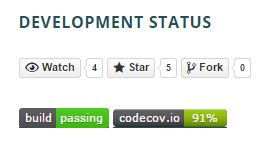
\includegraphics[width=7.011cm,height=3.863cm]{makingofmade113-img5.jpg}
}

Current development status
~

Any collaboration is welcomed. Github provides an excellent guide on
\href{https://help.github.com/articles/cloning-a-repository/}{how to
clone a repository}. Don{\textquoteright}t hesitate to contact if you
have any questions or comments about cloning MADE.

Finally, more technical posts are coming (any Java enthusiastic in the
room?).

{\bfseries
References:}

[1] Martin, Robert C. Clean Coder. mitp Verlags GmbH \& Co. KG, 2014.


\bigskip

\clearpage\section[The making of MADE (Part 6): Requirements by example
in Unit
Tests]{\href{http://www.velonuboso.com/made/2015/06/19/making-part-6-requirements-expressed-junit-tests/}{The
making of MADE (Part 6): Requirements by example in Unit Tests}}
June 19, 2015

Martin[1] defines three rules of TDD related to the nature of the tests:

\liststyleLxi
\begin{itemize}
\item \textstyleEmphasis{You may not write production code until you
have written a failing unit test.} 
\item \textstyleEmphasis{You may not write more of a unit test than is
sufficient to fail, and not compiling~is failing.} 
\item \textstyleEmphasis{You may not write more production code than is
sufficient to pass the currently~failing test.} 
\end{itemize}
MADE{\textquoteright}s tests follow these rules and reflect the
requirements by example using clear names and a standard
nomenclature.~This simplifies the documentation and allows the final
user (you)~to download and test every improvement.~Furthermore, I
{\textquotedblleft}do{\textquotedblright} believe that writing tests is
funny: instead of having one program, with TDD I can have~many small
programs that simply~work. If I have a new requirement I can write some
more programs, and all together are used to check the validity of the
software. Isn{\textquoteright}t it great?

MADE has currently 74 tests implemented. The rule followed in MADE for
the test names is to use readable names that explain the conditions and
the results of executing a method. For this reason, test~methods use
underscores and long names.

\textstyleStrongEmphasis{Running the tests (the boring way)}

If you are not afraid of the code and the shell, you can download the
source code and test the project with a maven goal.

{\textgreater} git clone https://github.com/raiben/made\newline
{\textgreater} cd made\newline
{\textgreater} mvn test

\textstyleStrongEmphasis{Running the tests (the easy~way)}

To simplify the test~of the different requirements (specially the future
ones, the interesting ones) I have created a project called
{\textquotedblleft}prettytestrunner{\textquotedblright}. It is just an
application that simply runs the tests and displays their names in a
pretty way (as requirements by example). Basically, if you run the
program, you get a list of real examples and their result in the
current version of MADE.

You can compile the program with the command {\textquotedblleft}mvn
assembly:assembly{\textquotedblright} but it is easier to download it
and execute it in a shell. Here is the
\href{https://www.dropbox.com/s/g95az0lv2tqn7b1/prettytestrunner-0.1-jar-with-dependencies.jar?dl=0}{link}~(courtesy
of Dropbox).

After downloading you only have to run:

{\textgreater} java -jar~prettytestrunner-0.1-jar-with-dependencies.jar

\textstyleStrongEmphasis{Listing the current tests}

(remember that the following names are extracted and transformed from
the tests names, so the syntax and grammar of the English may not be
correct in some cases).

Requisites of the World Integration\newline
1: OK -{\textgreater} AntMite is alive

Requisites of the Ant Mite\newline
1: OK -{\textgreater} GetName must return the name of the agent when
set\newline
2: OK -{\textgreater} GetName must return the default name when not
set\newline
3: OK -{\textgreater} GetFiniteStateAutomaton must return a valid
instance

Requisites of the Evaluator\newline
1: OK -{\textgreater} Prolog engine can be used\newline
2: OK -{\textgreater} Evaluator uses a list of events as input\newline
3: OK -{\textgreater} Evaluator must be configured with tropes

Requisites of the Event\newline
1: OK -{\textgreater} Event returns correct Predicate when two arguments
provided\newline
2: OK -{\textgreater} Event returns correct Predicate when no arguments
provided\newline
3: OK -{\textgreater} Event returns correct Predicate when one argument
provided\newline
4: OK -{\textgreater} Event returns correct Predicate with numbers and
strings

Requisites of the Events Log\newline
1: OK -{\textgreater} EventEntity getters must return set values\newline
2: OK -{\textgreater} DayLog getters must return set values\newline
3: OK -{\textgreater} EventsLog getters must return set values\newline
4: OK -{\textgreater} BoardEntity getters must return set values\newline
5: OK -{\textgreater} EventsLog is converted to json\newline
6: OK -{\textgreater} PositionEntity getters must return set
values\newline
7: OK -{\textgreater} CharacterEntity getters must return set
values\newline
8: OK -{\textgreater} fromJson must return EventsLog when Json is valid

Requisites of the Finite State Automaton\newline
1: OK -{\textgreater} run directs to first state when condition
accomplished and random lower than probability\newline
2: OK -{\textgreater} FiniteStateAutomaton is not correct when initial
state does not exist\newline
3: OK -{\textgreater} FiniteStateAutomaton is not correct when no
initial state is provided\newline
4: OK -{\textgreater} run directs to second state when first condition
did not accomplish\newline
5: OK -{\textgreater} FiniteStateAutomaton can use transitions\newline
6: OK -{\textgreater} getTargetStates must return states in
order\newline
7: OK -{\textgreater} FiniteStateAutomaton launches action of initial
state\newline
8: OK -{\textgreater} run directs to the same state when no condition
accomplish\newline
9: OK -{\textgreater} FiniteStateAutomaton is not correct when no states
are provided\newline
10: OK -{\textgreater} FiniteStateAutomaton is not correct when world is
not set\newline
11: OK -{\textgreater} run directs to the same state when no random
under probabilities

Requisites of the Map\newline
1: OK -{\textgreater} newMap: allCells must be land\newline
2: OK -{\textgreater} newMap: allCells must be empty\newline
3: OK -{\textgreater} getCellByPosition: cell retrieved by position and
retrieved by coords must be the same\newline
4: OK -{\textgreater} getPositionByCell: position retrieved by cell and
coords retrieved by cell must be the same\newline
5: OK -{\textgreater} moveCharacter: source with character and target
empty must move character to target\newline
6: OK -{\textgreater} getCellByCharacter: when character is moved to
target the returned cell must be the target\newline
7: OK -{\textgreater} getPositionsToMove: When movement is 1 and from 0x
0y then position 2x 2y must not be included\newline
8: OK -{\textgreater} getCell: allCells must have the same position than
the one used to get them\newline
9: OK -{\textgreater} removeCharacter: cell with character must remove
the character from the map\newline
10: OK -{\textgreater} putCharacter: putting the same character in two
cells must throw exception\newline
11: OK -{\textgreater} moveCharacter moving to a non empty location must
throw exception\newline
12: OK -{\textgreater} newMap: allCells must have different
position\newline
13: OK -{\textgreater} getCell: position out of bounds must be
moduled\newline
14: OK -{\textgreater} newMap: 20{\texttimes}20 must contain 400
cells\newline
15: OK -{\textgreater} getPositionsToMove When movement is 2 from 0x 0y
and obstacles then must not include unreachable cells\newline
16: OK -{\textgreater} putCharacter: in empty cell must put the
character\newline
17: OK -{\textgreater} moveCharacter: moving to the same location must
throw exception\newline
18: OK -{\textgreater} moveCharacter moving from an empty location must
throw exception\newline
19: OK -{\textgreater} putCharacter: in non empty cell must throw
exception\newline
20: OK -{\textgreater} getCellByCharacter: character in map must return
a cell\newline
21: OK -{\textgreater} getCellByCharacter character not in map must
return null\newline
22: OK -{\textgreater} getPositionsToMove: When movement is 2 and from
0x 0y then position 2x 2y must be included\newline
23: OK -{\textgreater} getPositionsToMove: When movement is 2 and from
0x 0y then position 18x 2y must be included\newline
24: OK -{\textgreater} getPositionsToMove: When movement is 2 and from
0x 0y then position 2x 18y must be included\newline
25: OK -{\textgreater} getPositionsToMove: When movement is 2 and from
0x 0y then position 18x 18y must be included

Requisites of the Random Number Factory\newline
1: OK -{\textgreater} getNextProbability returns a random number\newline
2: OK -{\textgreater} getNextProbability returns the sequence
provided\newline
3: OK -{\textgreater} getNextProbability returns a: number when seed is
0

Requisites of the String Util\newline
1: OK -{\textgreater} doubleTicksToQuote must convert each double tic to
quote

Requisites of the World\newline
1: OK -{\textgreater} World with no inhabitants must not return
pupulated list of inhabitants\newline
2: OK -{\textgreater} World with one inhabitant must return a pupulated
list of inhabitants\newline
3: OK -{\textgreater} World must have empty events when never
run\newline
4: OK -{\textgreater} World must set id 0 to the first
inhabitant\newline
5: OK -{\textgreater} World can tell a story about itselft\newline
6: OK -{\textgreater} World default time unit must be days\newline
7: OK -{\textgreater} World must set id to inhabitants\newline
8: OK -{\textgreater} World must set correlative ids to two correlative
inhabitants\newline
9: OK -{\textgreater} World must set a different id to each
inhabitant\newline
10: OK -{\textgreater} World must return 0 run time units when never
run\newline
11: OK -{\textgreater} World must use custom time unit when
configured\newline
12: OK -{\textgreater} World must be able to run a number of time
units\newline
13: OK -{\textgreater} World must have non empty events after
running\newline
14: OK -{\textgreater} AddInhabitant must insert an event when
called\newline
15: OK -{\textgreater} World must have events

\textstyleStrongEmphasis{References\newline
}[1] Martin, Robert C. Clean Coder. mitp Verlags GmbH \& Co. KG, 2014.

\textstyleStrongEmphasis{And remember, testing is better when a machine
can do it for you}



\bigskip

\clearpage\section[The making of MADE (Part 7): The
roadmap]{\href{http://www.velonuboso.com/made/2015/06/27/making-part-7-roadmap/}{The
making of MADE (Part 7): The roadmap}}
The following roadmap presents MADE short-term objetives (before the end
of july).

\liststyleLx
\begin{enumerate}
\item Narration engine: Writing events (to text). 
\item Inference engine: Inference of new events from the world events. 
\item Inference engine: Formalize the base predicates for the monomyth: 

\begin{enumerate}
\item Adventure. 
\item Hero. 
\item Shadow. 
\item Herald. 
\item Ally. 
\item Mentor. 
\item Shapeshifter. 
\item Shadow. 
\item Trickster. 
\end{enumerate}
\item Narration engine: Writing the monomyth predicates (to text). 
\item ABM engine: Components of the self-organisation: ABM Layer: 

\begin{enumerate}
\item Map. 
\item Agent. 
\item Passage of time. 
\end{enumerate}
\item ABM engine: Basic agent behavior as a {\textquotedblleft}living
thing{\textquotedblright}: 

\begin{enumerate}
\item Movement. 
\item Food and energy. 
\item Competitions. 
\item Collaborations. 
\item Relationships. 
\end{enumerate}
\item ABM engine: Inference from the world events to base predicates: 

\begin{enumerate}
\item Adventure. 
\item Hero. 
\item Shadow. 
\item Herald. 
\item Ally. 
\item Mentor. 
\item Shapeshifter. 
\item Shadow. 
\item Trickster. 
\end{enumerate}
\item Narration egine: generate personal stories and world story. 
\item EC engine: Assign fitness of the world{\textquoteright}s
backstories. 
\item EC engine: Define metrics of interest. 
\item EC engine: Extract execution parameters and codify~ the
chromosome. 
\item EC engine: Apply a canonical genetic algorithm to find the fittest
chromosome. 
\item EC engine: Define parameter configurations. 
\item Test the EC engine: 

\begin{enumerate}
\item Perform tests with different configurations. 
\item Analise the data. 
\item Extract conclussions. 
\end{enumerate}
\item Customization engine: Contextualise to different literary
settings: 

\begin{enumerate}
\item Futuristic 
\item Fantasy 
\item Steampunk 
\end{enumerate}
\item Customization engine: Conditions on the predicates in the
optimization phase. 
\item Customization engine: Conditions on predicates relevance in the
writing phase. 
\end{enumerate}



\bigskip

\clearpage\section[The making of MADE (Part 8): Component stack and
dataflow]{\href{http://www.velonuboso.com/made/2015/06/27/making-part-8-component-stack-dataflow/}{The
making of MADE (Part 8): Component stack and dataflow}}
June 27, 2015

MADE has two main applications (MADE optimizer and MADE simulator) and
five components (Customization engine, EC engine, ABM engine, Narration
engine and Inference engine).

\href{http://www.velonuboso.com/made/blog/wp-content/uploads/2015/06/MADEs-architecture-2.jpg}{
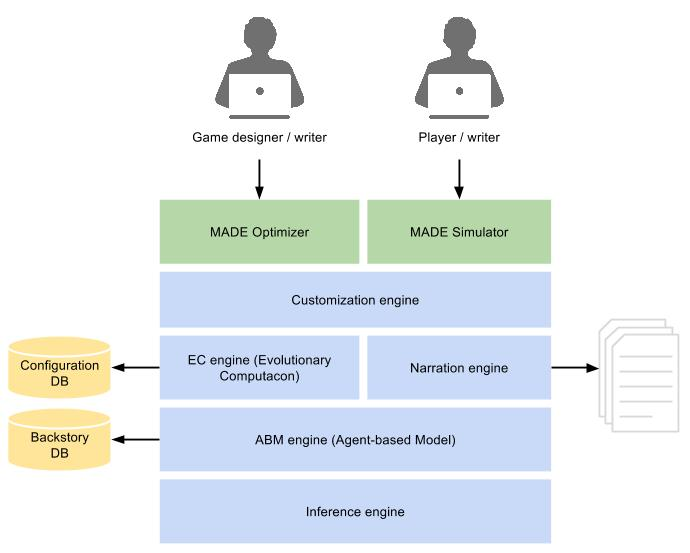
\includegraphics[width=16.955cm,height=13.598cm]{makingofmade113-img9.jpg}
}

MADE{\textquoteright}s component stack
Description of MADE{\textquoteright}s components:

\liststyleLix
\begin{itemize}
\item \textstyleStrongEmphasis{MADE Optimizer} can be used by a game
designer or a screenwriter. Its goal is to generate the configuration
for the correct emergence of the backstories when running the
simulator. It uses an hibrid EC-ABM approach (Evolutionary Computation
/ Agent-based Model) with and predicate-based inference engine that can
extract knowledge from the events. 
\item \textstyleStrongEmphasis{MADE Simulator} can be used by the
end-users (also a writer) and the videogame themselves, to simulate a
virtual world with backstories according to the parameters provided.
The backstories can be used directly by the narrator engine, that
produces a written story in natural language, or by third party
integration tools. 
\item The \textstyleStrongEmphasis{ABM Engine} provides a virtual world
generated according to given parameters and inhabited by autonomous
agents that interact to produce events. Those events form the world
backstories and can be translated to natural language. 
\item The \textstyleStrongEmphasis{Inference engine} is able to infer
new events from the events generated in a virtual world. It provides
high-level predicates related to tropes, archetypes and other literary
artefacts. 
\item The \textstyleStrongEmphasis{EC engine} is able to calculate the
fitness value for the world{\textquoteright}s backstories and uses an
Evolutionary Algorithm to find the configuration for the ABM engine
with the higher fitness value. 
\item The \textstyleStrongEmphasis{Narration engine} is used by MADE
Simulator and translates the world{\textquoteright}s backstories of a
simulation with the best configuration to written stories in natural
language. 


\bigskip
\end{itemize}
\href{http://www.velonuboso.com/made/blog/wp-content/uploads/2015/06/MADEs-architecture.jpg}{
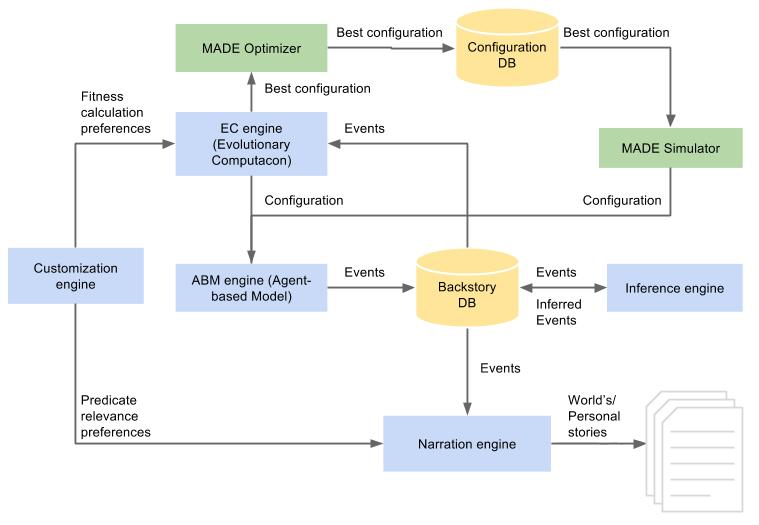
\includegraphics[width=16.928cm,height=11.723cm]{makingofmade113-img10.jpg}
}

MADE{\textquoteright}s data flow

\bigskip

\clearpage\section[The making of MADE (Part 9): Implementing a narration
engine]{\href{http://www.velonuboso.com/made/2015/07/11/making-part-7-testing-narration-engine/}{The
making of MADE (Part 9): Implementing a narration engine}}
July 11, 2015

As we mentioned before, the
\textstyleStrongEmphasis{world{\textquoteright}s events} and the
\textstyleStrongEmphasis{world{\textquoteright}s deductions} form,
together, the \textstyleStrongEmphasis{world{\textquoteright}s
backstories}. Each event or deduction is considered as a fact in the
virtual world, an is expressed as a \textstyleStrongEmphasis{logical
predicate}, with name, arguments and an interpretation, or a phrase,
expressed in natural language, that uses the arguments. Our assumption
is that, if we group the set of predicates (events and deductions)
present in the world{\textquoteright}s backstories, we order them by
date and concatenate all their interpretations, then we are able to
generate a very simple story.

\textstyleStrongEmphasis{Requirements:}

\liststyleLviii
\begin{enumerate}
\item The \textstyleStrongEmphasis{Narration engine} must receive the
\textstyleStrongEmphasis{world{\textquoteright}s backstories} to
produce a \textstyleStrongEmphasis{narration} in natural language. 
\item The \textstyleStrongEmphasis{Narration engine} can be
\textstyleStrongEmphasis{customized} to produce specific phrases from
specific predicates. This customization is independent from the
world{\textquoteright}s backstories. 
\end{enumerate}
\textstyleStrongEmphasis{Modelling by example:}

Precondition 1: The world{\textquoteright}s stories generated by the
simulator are:

{\ttfamily
Conflict (0, 0, {\textquotesingle}I\~nigo Montoya{\textquotesingle}, 1,
{\textquotesingle}the {\textquotedbl}six-fingered
man{\textquotedbl}{\textquotesingle},
{\textquotesingle}4{\textquotesingle}, {\textquotesingle}the death of
I\~nigo{\textquotesingle}s father{\textquotesingle})}

{\ttfamily
Helps (1, 0, {\textquotesingle}I\~nigo Montoya{\textquotesingle}, 2,
{\textquotesingle}Westley{\textquotesingle},
{\textquotesingle}20{\textquotesingle}, {\textquotesingle}his plan to
enter into the castle.{\textquotesingle})}

Precondition 2: The customization file must include the rules to
generate the desired narration:

Post-condition: The narration generated must be:
{\textquotedblleft}\textstyleEmphasis{The day 0, there was a conflict
between I\~nigo Montoya and the {\textquotedblleft}six-fingered
man{\textquotedblright} because of the death of
I\~nigo{\textquoteright}s father. The day 1, I\~nigo Montoya helped
Westley with his plan to enter into the castle.}{\textquotedblright}

\textstyleStrongEmphasis{Implementation:}

The \textstyleEmphasis{class diagram in figure 1} describes the Narrator
class and its components. Narrator implements INarrator interface and
uses an EventsLogEntity and and ICustomization.

{\centering
\href{http://www.velonuboso.com/made/blog/wp-content/uploads/2015/07/classcom_1_1velonuboso_1_1made_1_1core_1_1narration_1_1implementation_1_1_narrator__coll__graph.jpg}{
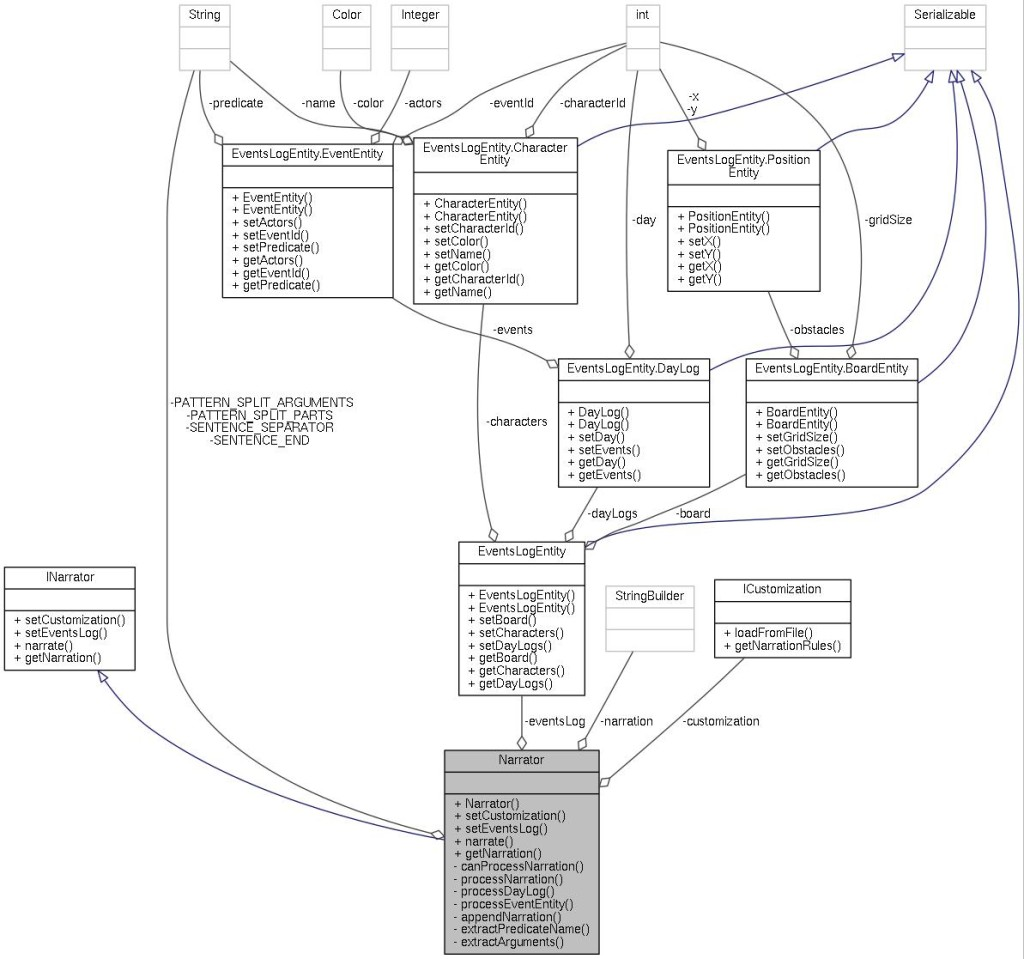
\includegraphics[width=17.515cm,height=16.404cm]{makingofmade113-img11.jpg}
}Figure 1: Narrator class sub-components
\par}

The \textstyleStrongEmphasis{Customization} class is constructed using a
json with an array of predicate interpretations (see example
\textstyleEmphasis{monomyth\_narration\_rules\_en.json}):

{\ttfamily
[}

{\ttfamily
~~~ \{}

{\ttfamily
~~~~~~~ {\textquotedbl}predicateName{\textquotedbl}:
{\textquotedbl}Conflict{\textquotedbl},}

{\ttfamily
~~~~~~~ {\textquotedbl}\_help{\textquotedbl}: {\textquotedbl}day, id\_0,
name\_0, id\_1, name\_1, source\_of\_conflict\_id,
source\_of\_conflict\_name{\textquotedbl},}

{\ttfamily
~~~~~~~ {\textquotedbl}numberOfArguments{\textquotedbl}: 7,}

{\ttfamily
~~~~~~~ {\textquotedbl}naturalLanguageTemplate{\textquotedbl}:
{\textquotedbl}The day \{0\}, there was a conflict between \{2\} and
\{4\} because of \{6\}{\textquotedbl}}

{\ttfamily
~~~ \}, \{}

{\ttfamily
~~~~~~~ {\textquotedbl}predicateName{\textquotedbl}:
{\textquotedbl}Helps{\textquotedbl},}

{\ttfamily
~~~~~~~ {\textquotedbl}\_help{\textquotedbl}: {\textquotedbl}day, day,
id\_0, name\_0, id\_1, name\_1, source\_of\_help\_id,
source\_of\_help\_name{\textquotedbl},}

{\ttfamily
~~~~~~~ {\textquotedbl}numberOfArguments{\textquotedbl}: 7,}

{\ttfamily
~~~~~~~ {\textquotedbl}naturalLanguageTemplate{\textquotedbl}:
{\textquotedbl}The day \{0\}, \{2\} helped \{4\} with
\{6\}{\textquotedbl}}

{\ttfamily
~~~ \}}

{\ttfamily
]}

A narrator uses this customization and an
\textstyleStrongEmphasis{EventsLogEntity} to produce the narration. The
EventsLogEntity has the structure displayed in figure 2.

{\centering
\href{http://www.velonuboso.com/made/blog/wp-content/uploads/2015/07/classcom_1_1velonuboso_1_1made_1_1core_1_1common_1_1entity_1_1_events_log_entity__coll__graph.jpg}{
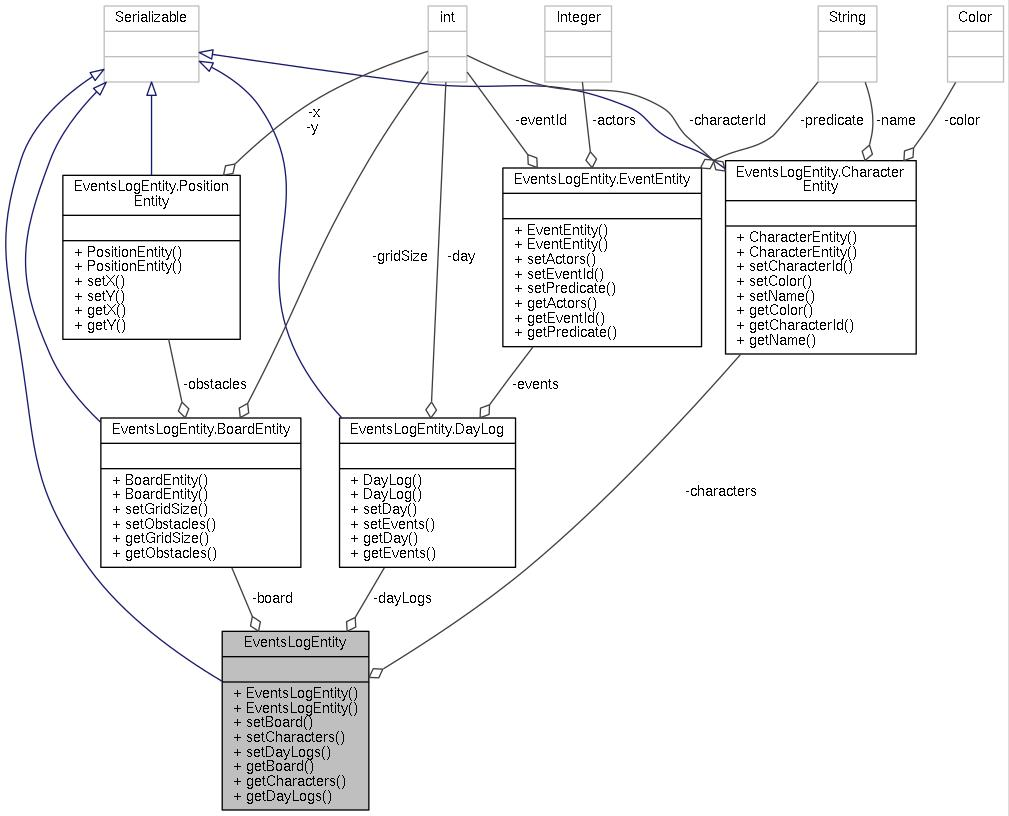
\includegraphics[width=17.544cm,height=14.196cm]{makingofmade113-img12.jpg}
}Figure 2: \textstyleEmphasis{EventsLogEntity class sub-components}
\par}

As result, the narrator generates the following output:

\textstyleEmphasis{The day 0, there was a conflict between I\~nigo
Montoya and the {\textquotedblleft}six-fingered man{\textquotedblright}
because of the death of I\~nigo{\textquoteright}s father. The day 1,
I\~nigo Montoya helped Westley with his plan to enter into the castle.}

More tests can be found in
\textstyleEmphasis{NarrationRuleEntityTest.java} and
\textstyleEmphasis{MonomythNarrationIntegrationTest.java}. Feel free to
visit the source code and comment in the blog. In the next posts we
will study some more interesting predicates.



{\textquotedblleft}Hello, My name is Inigo Montoya. You killed my
father. Prepare to die{\textquotedblright}, by
\href{https://www.flickr.com/photos/7815007@N07/}{Ken Whytock}. License
CC BY-NC 2.0
\clearpage\section[The making of MADE (Part 10): Looking for heroes (the
monomyth)]{\href{http://www.velonuboso.com/made/2015/07/12/making-part-10-heroes-the-problem/}{The
making of MADE (Part 10): Looking for heroes (the monomyth)}}
July 12, 2015

In narratology and comparative mythology, the monomyth (or the
hero{\textquoteright}s journey) is a common literary pattern found in
classic myths but also in contemporary book, films and comics. Firstly
introduced by Campbell in 1949 in~ \textit{The Hero with a Thousand
Faces} [1], the monomith is summarised as
{\textquoteleft}\textstyleEmphasis{A hero ventures forth from the world
of common day into a region of supernatural wonder: fabulous forces are
there encountered and a decisive victory is won: the hero comes back
from this mysterious adventure with the power to bestow boons on his
fellow man}{\textquoteleft}.

  [Warning: Image ignored] % Unhandled or unsupported graphics:
%\includegraphics[width=10.53cm,height=10.583cm]{makingofmade113-img14}
 

The Hero{\textquoteright}s Journey, from
\href{https://en.wikipedia.org/wiki/File:Heroesjourney.svg}{the
wikipedia}. Public domain

We{\textquoteright}ll talk more about the monomyth in future post. By
now, we only introduce the concept and use some of the definitions by
Vogler [2] to \textstyleStrongEmphasis{guide next
MADE{\textquoteright}s requisites related to the deduction and
narration engine}. Remenber that, in
\href{http://www.velonuboso.com/made/2015/06/14/making-part-3-worlds-facts-worlds-deductions-worlds-backstories/}{The
making of MADE (Part 3)}, we defined the world{\textquoteright}s
deductions as \textstyleEmphasis{if-then sentences}.

Deductions can be expressed as
Expression[200B?]0[200B?][200B?]$\rightarrow
$Expression[200B?]1[200B?][200B?], where
Expression[200B?]0[200B?][200B?]~is the premise and
Expression[200B?]1[200B?][200B?]~the conclusion, and both are logical
expressions on predicates from the
\textstyleStrongEmphasis{world{\textquoteright}s facts} and from the
\textstyleStrongEmphasis{world{\textquoteright}s deductions}.

Following [3], Vogler defined in 8 archetypes in the
\textstyleEmphasis{monomyth}:

\liststyleLvii
\begin{enumerate}
\item \textstyleStrongEmphasis{The hero} is the central figure of the
journey. \textstyleEmphasis{{\textquoteleft}The hero is the person who
goes out and achieves great deeds on behalf of the group, tribe, or
civilization{\textquoteright}}. 
\item \textbf{The mentor} is the hero{\textquoteright}s guide and
protector. 
\item \textbf{The threshold Guardians} are the the forces that the hero
must overcome along the journey, including enemies and own fears. 
\item \textbf{The herald} is the caller to the adventure for the hero. 
\item \textbf{The shapeshifters} are characters who change along the
journey. 
\item \textbf{The shadow }is the villain, the dark side. 
\item \textbf{The allies} help the hero through the journey. 
\item \textbf{The tricksters} are mischief-makers. 
\end{enumerate}
The \textstyleEmphasis{monomyth} can be found in a multitude of movies,
TV shows, books, songs, and videogames, from \textstyleEmphasis{Skyrim}
and \textstyleEmphasis{Mass effects} [4] to \textstyleEmphasis{The
legend of Zelda} [5] and \textstyleEmphasis{Assassin{\textquoteright}s
creed }[6]. In future posts, we will model these archetypes as
predicates in the world{\textquoteright}s deductions, and
\textstyleStrongEmphasis{MADE will logically infer them from simple
predicates}, since one of the the main goals of our project is to
generate \textstyleStrongEmphasis{interesting backstories}.

\textstyleStrongEmphasis{References}

[1] Campbell, Joseph. \textit{The Hero with a Thousand Faces}.
Princeton: Princeton University Press, 1949. p.23\newline
[2] Vogler, Christopher. \textit{The Writer{\textquoteright}s journey}.
Michael Wiese Productions, 2007.\newline
[3] Vogler, Christopher. (2015, July 12). Hero{\textquoteright}s journey
[Online]. Available:
www.thewritersjourney.com/hero{\textquoteright}s\_journey.htm\newline
[4] Knopf, Ehsan. \textstyleEmphasis{The Rationalist{\textquoteright}s
Spirituality: Campbell{\textquoteright}s Monomyth in Single-Player
Role-Playing Videogames Skyrim \& Mass Effect.} 2013.\newline
[5] Wrisinger, Carli.
{\textquotedblleft}\textit{Link{\textquotedblright} ing monomyth and
video games: how The Legend of Zelda connects myth to modern media}.
Diss. 2014.\newline
[6] Ngamgamol, Apirath. \textit{A NARRATIVE ANALYSIS OF
ASSASSIN{\textquoteright}S CREED GAMING SERIES}. Diss. National
Institute of Development Administration, 2014.

~



{\textquotedblleft}\href{http://www.deviantart.com/art/Skyrim-268746720}{Skyrim}{\textquotedblright}
by \href{http://super-cute.deviantart.com/}{Super-Cute} from
Deviantart.com

\bigskip

\clearpage\section[The making of MADE (Part 11): Predicate dependency
graph for the
archetypes]{\href{http://www.velonuboso.com/made/2015/07/18/making-part-11-predicate-dependency-graph-archetypes/}{The
making of MADE (Part 11): Predicate dependency graph for the
archetypes}}
A first~analysis of the archetypes in the \textstyleEmphasis{monomyth}
have a revealed the existence of simple predicates (base predicates)
that are used to deduce more complex predicates (archetypes). In our
mental diagram, we have the following predicate names and dependencies
in our \textstyleStrongEmphasis{world{\textquoteright}s deductions:}

\href{http://www.velonuboso.com/made/blog/wp-content/uploads/2015/07/descarga.jpg}{
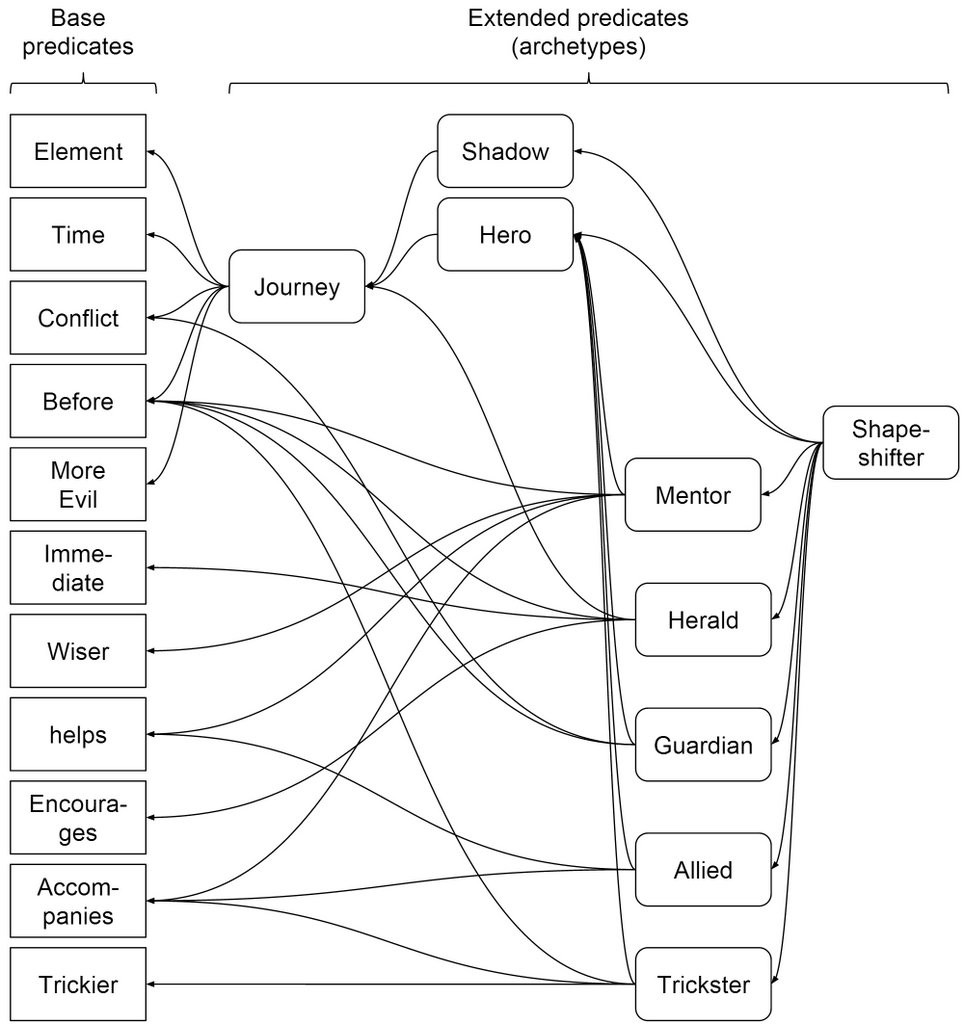
\includegraphics[width=14.229cm,height=15.109cm]{makingofmade113-img16.jpg}
}

Monomyth MADE World{\textquoteright}s deductions
Following this diagram, if we have very basic predicates (for example,
what is an element or when we consider that one moment is previous or
later to other) we are able to construct more complex predicates (our
archetypes).

For example, we can define the \textstyleEmphasis{journey} with two
\textstyleEmphasis{elements} (the future hero and his/her future
shadow, that will be more \textstyleEmphasis{evil}) and two
\textstyleEmphasis{conflicts} between them (In the first one one
element is the~\textstyleEmphasis{winner}, the evil, and in the second
one the other elements is the \textstyleEmphasis{winner}, the good
guy). Once we have a \textstyleEmphasis{journey}, we can deduce a
predicate that tell us who is the \textstyleEmphasis{hero} and who is
the \textstyleEmphasis{shadow}. Then, some more predicates can be
deduced: the \textstyleEmphasis{mentor}, the
\textstyleEmphasis{herald}, the \textstyleEmphasis{guardian}, the
\textstyleEmphasis{allied} and the \textstyleEmphasis{trickster} also
take part on the journey, by helping, encouraging~or accompanying the
hero along~the journey.

Let{\textquoteright}s keep in mind this diagram~although it may vary
along the definition process. To finish~the Step 3 of our roadmap
({\textquotedblleft}\textstyleEmphasis{Inference engine: Formalize the
base predicates for the monomyth}{\textquotedblleft}) it could be good
to move forward to step 5 ({\textquotedblleft}\textstyleEmphasis{ABM
engine: Components of the self-organisation: ABM
Layer}{\textquotedblleft})~and try to briefly define a virtual world
able to generate~the set of predicates in the world{\textquoteright}s
deductions~that lead to all the predicates defined in the
world{\textquoteright}s events.


\bigskip

\clearpage\section[The making of MADE (Part 12): A simple, but powerful
virtual
world]{\href{http://www.velonuboso.com/made/2015/07/18/making-part-12-simple-powerful-virtual-world/}{The
making of MADE (Part 12): A simple, but powerful virtual world}}
July 18, 2015

In previous designs of MADE [1] our virtual world was inhabited by
virtual rats: {\textquoteleft}\textstyleEmphasis{A number of rats live,
eat, reproduce, compete for food and death within the walls of the
Invisible University of Ankh-Morpork . As the University professors,
these rats are very vindictive and territorial}{\textquoteleft}.

We have analysed the design of these agents~and discovered that they~are
not valid for our new implementation of MADE. They
don{\textquoteright}t implement a feeling-driven behaviour, and without
affectivity networks we cannot reach archetypes related to love, hate,
fear or shame{\dots} We need to design a simpler but more powerful
behaviour{\dots} let{\textquoteright}s remove
the~\textstyleEmphasis{discworld}~context and let the
\href{http://www.velonuboso.com/made/2015/06/27/making-part-8-component-stack-dataflow/}{Narration
and Customization engines} contextualize the backstories to the target
literary setting~.

\subsection{The rules of the virtual world}
The elements of the virtual world are the map, the pieces, the colours
spots and the turns. Each piece will try to maximize its own joy ~and
also its friends{\textquoteright} joy. In this virtual world, pieces
will compete and collaborate to reach their desired colour :-).

\subsubsection{Map and pieces}
\liststyleLi
\begin{itemize}
\item The world map is a board of 10{\texttimes}10 square cell. 
\item There are three kind of pieces: circle, triangle and square. 
\item Each piece can occupy only one cell. Every can be occupied by only
one piece. 
\item Every piece has a border colour (desired) and a background colour
(actual). 
\end{itemize}
\subsubsection{Turns}
\liststyleLxii
\begin{itemize}
\item Every turn, each piece can move to an adjacent empty cell. 
\item A piece can move other piece and occupy its cell under certain
conditions*. Both cells change their background colour (actual) to
their opposite. 
\item The priority of movements is randomly calculated each turn 
\item Every turn, the background colour (actual) of every cell changes
randomly a given percentage (\%). 
\item Every (n) turns, a random colour spot appears into a random cell.
The spot disappears before a new spot is placed. 
\end{itemize}
\subsubsection{Colours}
\liststyleLxiii
\begin{itemize}
\item When a piece is over a cell with a colour spot, the background
colour (actual) turns to the spot colour in a given percentage (\%). 
\item A piece can transfer a given percentage (\%) of background colour
(actual) to a target piece if its background colour (actual) gets
closer to the border colour (desired). 
\item A piece can steal a given percentage (\%) of background colour
(actual) to a target piece under certain conditions*. 
\end{itemize}
* A circle can move/steal to a triangle. A triangle can move/steal to a
square. A square can move/steal to a circle.

\subsubsection{Strategies}
Every piece{\textquoteright}s turn can consist in one of the following
strategies:

\liststyleLxiv
\begin{enumerate}
\item Skip turn 
\item Move closer to other piece 
\item Move away from other piece 
\item Move closer to a spot 
\item Move away from a spot 
\item Move other piece 
\item Transfer colour to other piece 
\item Steal colour from other piece 
\item Move in a random direction 
\end{enumerate}
\subsubsection{Feelings-based behaviour}
Every piece has 8 basic feelings, based in the works of Plutchik in
[2].~In MADE, every feeling can have a real value, from 0 to 1:

\textstyleStrongEmphasis{Joy / sadness}

Every piece has a joy~level, proportional to:

\liststyleLxv
\begin{itemize}
\item The similarity between the border colour (desired) and background
colour (actual), 
\item the similarity between the border colour (desired) and background
colour (actual) of its friends. 
\item and the difference~between the border colour (desired) and
background colour (actual) of its enemies. 
\end{itemize}
In its turn, the piece will try to increase its joy level by changing
its colour or its friends colour, by applying any of the nine
strategies.

\textstyleStrongEmphasis{Trust / disgust (regarding to every other
piece)}

Every piece has a grade of trust / disgust~related to every other piece.
The trust~on the target piece is directly proportional to:

\liststyleLxvi
\begin{itemize}
\item The similarity of the border colour (desired), 
\item the similarity of the background colour (actual), 
\item and the similarity of the shape 
\end{itemize}
The friends of a piece are all the pieces that the piece trust on~over a
certain value.~The enemies of a piece are all the pieces that the piece
trust on~bellow~a certain value.

The trust / disgust levels will be used to calculate the joy level of
every piece.

\textstyleStrongEmphasis{Fear}

Every piece has a grade of fear proportional to the joy level that it
will get due to the action of other pieces. When this level is high, it
will apply the strategy 3 {\textquotedblleft}Move away from other
piece{\textquotedblright}.

\textstyleStrongEmphasis{Surprise}

Every piece has a grade of surprise~that will be high when a piece
changes suddenly of colour. The strategy applied will be ~9
{\textquotedblleft}Move in a random direction{\textquotedblright}.

\textstyleStrongEmphasis{Anticipation}

Every piece has a grade of anticipation that will be high when a piece
can experiment~a big increment of joy. The strategies applied can be
all but 1, 3 and 5 (skip turn and move away).

\href{http://www.velonuboso.com/made/blog/wp-content/uploads/2015/07/player1.jpg}{
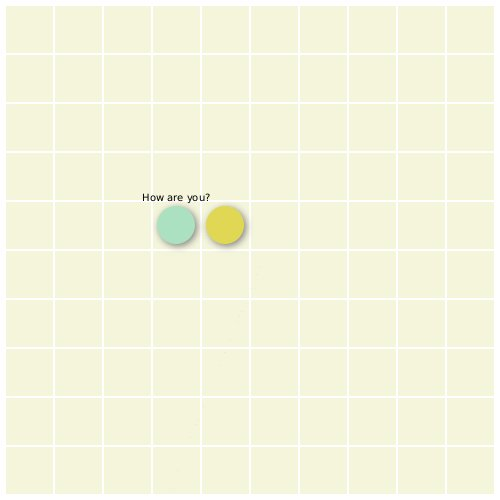
\includegraphics[width=13.282cm,height=13.282cm]{makingofmade113-img17.jpg}
}

Sample of MADE Player project execution
Do you like the virtual world? How would you call it? Suggestions are
accepted.

\textstyleStrongEmphasis{References}

[1] Garcia-Ortega, Ruben H., et al. {\textquotedblleft}My life as a sim:
evolving unique and engaging life stories using virtual
worlds.{\textquotedblright} \textit{ALIFE 14: The Fourteenth Conference
on the Synthesis and Simulation of Living Systems}. Vol. 14. 2014.

[2]~Plutchik, Robert. {\textquotedblleft}Emotions: A general
psychoevolutionary theory.{\textquotedblright} \textit{Approaches to
emotion} 1984 (1984): 197-219.


\bigskip

\clearpage\section[The making of MADE (Part 13): Feelings{}-driven IA
for our
agents]{\href{http://www.velonuboso.com/made/2015/07/24/making-part-13-feelings-driven-ia-agents/}{The
making of MADE (Part 13): Feelings-driven IA for our agents}}
July 24, 2015

In previous posts we defined
\href{http://www.velonuboso.com/made/2015/07/18/making-part-12-simple-powerful-virtual-world/}{the
rules of virtual world} and the
\href{http://www.velonuboso.com/made/2015/07/18/making-part-11-predicate-dependency-graph-archetypes/}{world{\textquoteright}s
deductions} that we will need for the emergence of different archetypes
related to the \textstyleEmphasis{monomyth}. We need to design the IA
of our pieces in order to make them compete/cooperate and generate
conflicts.~Currently, the most extended and popular~technique to define
IAs in~videogames is called
{\textquotedblleft}\textstyleEmphasis{behaviour
tree}{\textquotedblright} and is used by game engines like Unreal or
Unity. As defined by Llans\'o in [1],
\textstyleEmphasis{{\textquoteleft}Behaviour Trees are an expressive
mechanism that let designers create complex behaviours by defining an
AI driven by goals, in which complex~behaviours can be created
combining simpler ones using a hierarchical approach{\textquoteright}}.

Our behaviour tree reflects the feelings-based philosophy described in
previous posts:

\href{http://www.velonuboso.com/made/blog/wp-content/uploads/2015/07/piece_behaviour_tree_1.jpg}{
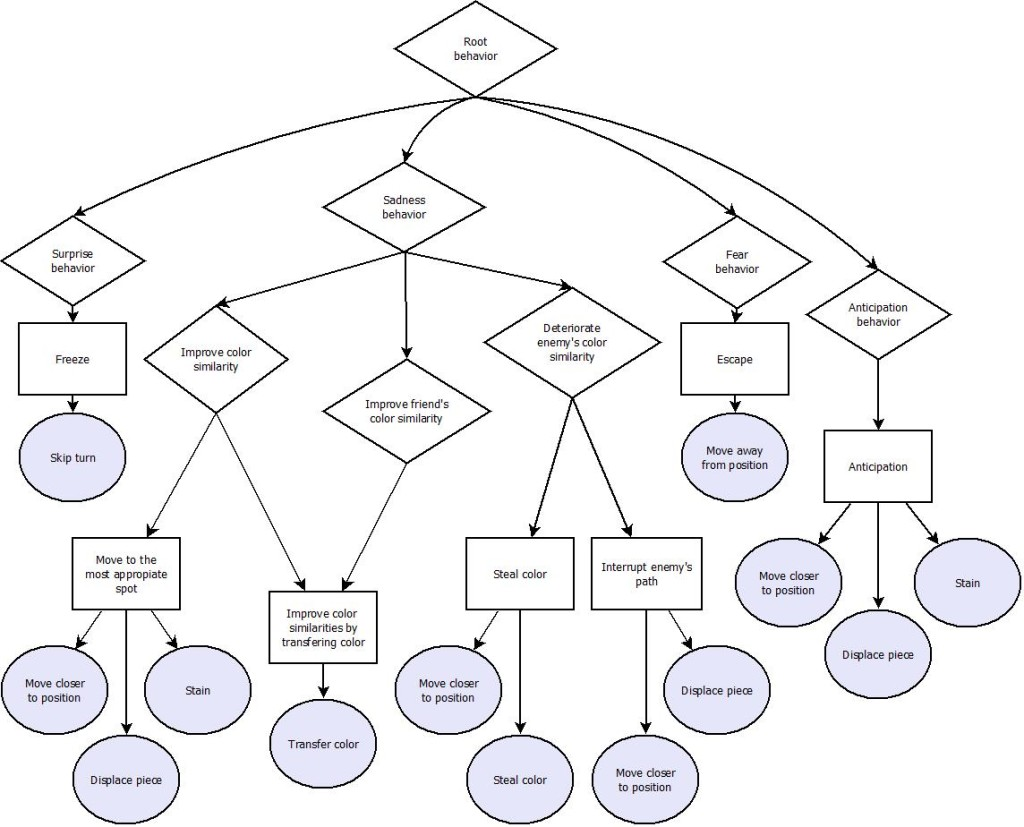
\includegraphics[width=16.955cm,height=13.702cm]{makingofmade113-img18.jpg}
}

MADE Piece{\textquoteright}s behaviour tree
Our next step is to define the predicates that will form the
world{\textquoteright}s stories with this behaviour tree and try to
define the inference rules to obtain the \textstyleEmphasis{monomyth}
base predicates.
\end{document}
